%!TEX output_directory = ./aux/

\documentclass[pt,disc,oneside]{ufscpgeasthesis}

\usepackage[utf8]{inputenc}

\usepackage[font=small,format=plain,labelfont=bf,up,textfont=it,up]{caption}
\usepackage[dvipsnames]{xcolor}
\usepackage[export]{adjustbox}
\usepackage{subfigure}
\usepackage{listings}
\usepackage{supertabular}
\usepackage{colortbl}
\usepackage{color}
\usepackage{listings}
\usepackage{float}
\usepackage{textcomp}

\newcommand{\defsigla}[2] {(#1 - \concept{#2})\sigla{#1}{#2} }
\newcommand{\defsimbolo}[2] {#1\simbolo{#1}{#2}}
\newcommand{\defconceito}[3] {\concept{#1}#2#3\conceito{#1}{#3}}
\newcommand{\defequacao}[2] {{\label{#1}}\equacao{\ref{#1}}{#2}}
\newcommand{\comentario}[1] {}
\newcommand{\rascunho}[1] {}
\newcommand{\foralugar} {}
\newcommand{\desc}[1] {\multicolumn{2}{|l|}{#1} \\}
\newcommand{\itemtt}[1] {\textbf{#1}}
\newcommand{\concept}[1] {\textit{#1}}
\newcommand{\msetf}[1] {\mathcal{#1}}
\newcommand{\mfuncf}[1] {\mathfrak{#1}}
\newcommand{\mvecsf}[1] {#1}
\newcommand{\mvar}[2] {#1\negthinspace{\scriptstyle{#2}}}
\newcommand{\mssubs}[1] {_{\negthickspace{\scriptscriptstyle{#1}}}}
\newcommand{\mvect}[1] {\overrightarrow{\mvecsf{#1}}}
\newcommand{\mvecs}[2] {\overrightarrow{\mvecsf{#1}}\mssubs{#2}} 
 
\setlength{\parskip}{0.30 cm}
\setlength{\parindent}{1.25 cm}
\lstset{numbers=left, stepnumber=1, firstnumber=1, numberstyle=\tiny, extendedchars=true, breaklines=true, frame=tb, basicstyle=\scriptsize, stringstyle=\ttfamily, showstringspaces=false}

\university        {Universidade Federal de Santa Catarina}
\address           {Florianópolis}
\institute         {}
\department        {Departamento de Informática e Estatística}
\program           {Curso de Ciência da Computação}
\majorfield        {Ciência da Computação}
\title             {Simulação de um Empreendimento do Ramo Alimentício}
\discipline        {Modelagem e Simulação de Sistemas}
\year              {2018}
\month             {Agosto}
\author            {Bruno Bonotto \\ Fabíola Maria \\ João Vicente}
\adviser           {Rafael Luiz Cancian}
\coadviser         {}

\begin{document}

	\frontpage
	\presentationpage
	\tableofcontents

	\resumo

		Atualmente, a compreensão de características do estabelecimento e também a identificação de melhorias se tornou importante para o setor alimentício.
		Isso ocorre em razão da ampla concorrência nesse setor, assim, os empresários desse ramo devem investir corretamente o capital disponível, com o intuito de agradar os clientes e se possível atrair novos.
		Dessa forma, dois empresários do ramo alimentício identificaram a necessidade de aplicar em seu empreendimento de forma mais bem planejada.
		A maneira que melhor lhes chamou a atenção para isso foi a realização de simulações que pudessem ``predizer'' quais seriam os possíveis retornos de suas ideias.
		Dada a restrição no valor disponível para realização de alterações no restaurante, foram propostas algumas possíveis melhorias, sendo as que apresentaram melhores chances de bom retornos as seguintes: aumentar o número de cozinheiros para reduzir o tempo de espera dos clientes ou remover uma certa quantidade de mesas para a construção de um palco que seria utilizado para atrair mais clientes ao restaurante.
		Após a realização de um modelo que fosse suficientemente capaz de representar as características do restaurante real, certas modificações foram realizadas para avaliar o impacto de determinadas aplicações.
		Os resultados mostraram que os principais fatores que influenciavam no número de clientes atendidos era tanto o número de cozinheiro quanto o de atendentes.
		Dessa forma, notou-se que o impacto causado com apenas o aumento no número de cozinheiros era mínimo, uma vez que não haviam atendentes o suficiente para anotar os pedidos dos clientes.
		Devido à essa característica do modelo, foi possível avaliar o impacto no número de clientes atendidos quando aumentado tanto o número de cozinheiros quanto de atendentes e, nesse caso, o resultado foi um aumento de quase 200\% no número de clientes atendidos.
		Outra característica interessante do modelo, obtida através da análise do impacto do número de mesas na quantidade de clientes atendidos, mostrou que as mesas de fato estavam sendo subutilizadas.
		Isso ficou claro quando avaliados os cenários em que 40\% das mesas foram retiradas, uma vez que essa remoção não impactava em quase nada no número de clientes atendidos.
		Assim, foi possível concluir que a contratação de novos cozinheiros não seria necessário para que os empresários atingissem seus objetivos, mas que a remoção de mesas em prol da construção de um palco, estatisticamente, tinha maiores probabilidades de prover bons resultados futuros.

   \begin{keywords}
      Modelagem e Simulação de Sistemas; Estatística; Projeto de Experimentos.
   \end{keywords}

   \mainmatter

	\chapter{Introdução}
	\label{cap:introducao}

		Segundo \cite{Pereira2012}, os investimentos com modificações de produtos, processos, tecnologias e arranjos físicos são altos e arriscados.
		Na tentativa de reduzir fracassos devido à previsões enviesadas e sem fundamento estatístico, faz-se necessário o uso de simulações.
		Simular a aplicação de novos agentes no sistema permite uma visualização mais detalhada do funcionamento do organismo.
		Também, através de modelos computacionais, permite a realização de testes com cenários alternativos para indicar soluções a baixo custo.

		Para aumentar a probabilidade de sucesso em futuros investimentos, dois empresários precisam estimar com precisão os efeitos de determinadas ações.
		Neste sentido, o presente trabalho desenvolve um modelo de simulação para atender tal demanda.
		O empreendimento ao qual se propõe processos de simulações pertence ao setor alimentício, tratando-se de um restaurante.

		Diversas ideias de como melhorar o negócio foram discutidas entre os proprietários.
		No entanto, chegou-se à conclusão de que apenas duas delas possuem de fato potencial para aumentar os lucros.
		Uma consiste em contratar quatro novos cozinheiros e, além disso, reformar a cozinha à fim de permitir melhor utilização dos recursos.
		A outra, por sua vez, consistem em remover 40\% das mesas em função da construção de um palco para apresentações ao vivo.
		Porém, o fundo destinado ao desenvolvimento do negócio é limitado e, por conta disso, ambas as ideias não podem ser realizadas simultaneamente.
		Assim, este trabalho se propões à realizar simulações para ambas as possibilidades abordadas pelos proprietários do negócio.

		A simulação do estabelecimento, e os possíveis cenários, foi modelada e executada através da ferramenta Arena \cite{Arena}.
		A partir dos resultados obtidos e com as apropriadas análises estatísticas, foi possível auxiliar os empresários na tomada de decisão.
		Assim, reduziu-se a propensão à investimentos onerosos.
		Maiores detalhes são mostrados no Capítulo \ref{cap:desenvolvimento}.

		\section{Objetivos}
		\label{sec:objetivos}

			\subsection{Objetivos Gerais}
			\label{subsec:objetivos_gerais}

				Os objetivos gerais deste projeto consiste em simular um restaurante, avaliar quais os possíveis impactos advindos de determinados investimentos e, também, servir de auxílio na tomada de decisão sobre em qual investimento aplicar os fundos de desenvolvimento.
				Neste sentido, trata-se de avaliar estatisticamente a influência, em quantidade de clientes atendidos, causada pela contratação de quatro novos cozinheiros.
				Assim como avaliar o impacto no número de clientes atendidos caso retirado 40\% das mesas para construção de um palco.

			\subsection{Objetivos Específicos}
			\label{subsec:objetivos_especificos}

				\begin{itemize}
					\item Identificar as distribuições de probabilidade a partir de dados coletados.
					\item Empregar uma ferramenta de simulação para modelagem do negócio e desenvolver o modelo correspondente.
					\item Aplicar técnicas para verificação e validação do modelo de simulação.
					\item Simular o impacto no número de clientes atendidos considerando a contratação de quatro novos funcionários.
					\item Simular o impacto no número de clientes atendidos pela remoção de 40\% das mesas.
					\item Analisar os resultados obtidos nas simulações usando uma técnica estatística apropriada.
					\item Avaliar qual a melhor forma de investimento que cumpre com os objetivos dos empresários.
				\end{itemize}

		\section{Hipóteses de Pesquisa}
		\label{sec:hipoteses}

			São apresentadas abaixo, as duas hipóteses estatísticas sobre as quais são realizadas análises estatísticas.
			Além disso, são apresentados em sequência os fatores que influenciam a métrica de desempenho avaliada, ou seja, o número de vendas do empreendimento.

			\begin{itemize}
				\item{\textbf{Hipótese 1:}} Contratar quatro cozinheiros auxilares duplicaria o número de pessoas atendidas.
				\item{\textbf{Hipótese 2:}} Retirar 40\% das mesas não interfere no número de pessoas atendidas.
				\item{\textbf{Fatores de influência a métrica mensurada:}}
				\begin{enumerate}
					\item Tempo de chegada de clientes.
					\item Tempo de preparo das refeições.
					\item Tempo de alimentação dos clientes.
				\end{enumerate}
			\end{itemize}

		\section{Organização do Projeto}
		\label{sec:organizacao}

			O restante deste documento está organizado da seguinte maneira: o Capítulo \ref{cap:fundamentacao} apresenta as principais soluções existentes para o problema sendo tratado, bem como as técnicas utilizadas no projeto sendo desenvolvido.
			Assim, consiste em apresentar os principais aspectos de outros trabalhos no mesmo contexto do projeto sendo desenvolvido, os aspectos sobre simulação de sistemas e síntese estatística utilizados neste projeto, os principais aspectos sobre a inferência estatística e o projeto de experimentos utilizados neste trabalho.
			No Capítulo \ref{cap:desenvolvimento} são descritas, em detalhes, cada uma das etapa do projeto de simulação de sistemas que foi desenvolvido.
			Para isso, são definidos os propósitos e objetivos do projeto, avaliados os aspectos relacionados aos recursos necessários à sua execução e especificado como o sistema funciona.
			Ainda, é especificado como foi feita a coleta e o tratamento de dados para a simulação, como o modelo foi desenvolvido no Arena e qual o processo de verificação e validação do modelo utilizados e como foi projetado o conjunto de experimentos que permitam atender os objetivos especificados.
			Por fim, são realizadas inferências estatísticas sobre os resultados da simulação que, por sua vez, são relatadas de forma organizada e sistematizada.
			As conclusões são discutidas na seção seguinte.

	\chapter{Fundamentação Teórica}
	\label{cap:fundamentacao}

		\section{Simulação de Sistemas}
		\label{sec:simulacao}

			Em \cite{Distribuicoes} simulação refere-se a uma ampla coleção de métodos e aplicações para imitar o comportamento de um sistema real.
			Geralmente, a simulação é realizada por um computador através de um software adequado.
			Outra definição de simulação de sistemas, esta fornecida em \cite{Freitas}, aborda apenas os métodos que utilizam técnicas matemáticas.
			No entanto, devido à demanda de bastante conhecimento e aprofundamento em modelos matemáticos complexos, sua aplicação para determinados problemas se torna completamente inviável.
			Algumas vezes, para que ainda seja possível uma modelagem matemática, o modelo proposto sofre certas simplificações.
			O modelo estudado pela simulação consiste, basicamente, na criação de uma história artificial baseada no sistema real, onde pressupõe-se uma série de simplificações.
			Tais simplificações, usualmente, tomam a forma de relações matemáticas ou lógicas.
			Ainda, além dos modelos já mencionados, existem os modelos lógico (matemático) e físico.
			O modelo lógico consiste em apenas um conjunto de aproximações e suposições, tanto estruturais quanto quantitativas, sobre o modo como o sistema faz ou irá funcionar.
			Já o físico modela a realidade e pode ser útil para diversas áreas, principalmente engenharias.
			Um modelo de simulação é dividido em diversas partes e para que se possa compreendê-lo é necessário entender cada uma delas \cite{Freitas}:
 
			\begin{itemize}
				\item{\textbf{Entidades:}} são objetos dinâmicos da simulação, geralmente são criados, movidos e descartados.
				Podem tanto serem criados pelo usuário quanto automaticamente pelo simulador.
				Ainda, uma entidade pode modificar o estado da outra ou até mesmo do sistema.
				\item{\textbf{Atributos:}} são as características das entidades, ou também são valores específico para cada uma delas, indicando sua individualidade.
				\item{\textbf{Variáveis:}} são informações que refletem diretamente a característica do sistema independentemente de quantos ou quais tipos de entidades podem estar por perto.
				\item{\textbf{Recursos:}} representam pessoas, equipamentos ou espaços que possuem um tamanho limite.
				Entidades podem competir umas com as outras por um determinado recurso.
				\item{\textbf{Filas:}} guardam um conjunto de entidades que estão aguardando por um mesmo recurso enquanto o mesmo está sendo utilizado por outra(s) entidade(s).
				\item{\textbf{Acumuladores estatísticos:}} obtém as medidas de desempenho, é uma parte essencial para que seja possível fazer análises dos dados.
				\item{\textbf{Eventos:}} um evento é algo que acontece em um instante de tempo de simulação e modifica atributos, variáveis ou acumuladores estatísticos.
				\item{\textbf{Tempo de Simulação:}} é valor de tempo atual da simulação.
				Ao contrário do tempo real, o tempo de simulação não flui continuamente, podendo ser expandido e comprimido.
				\item{\textbf{Iniciar e finalizar:}} é importante saber que para fazer uma simulação é necessário iniciar e terminar e, assim, identificar e analisar os dados obtidos.
			\end{itemize}

			A modelagem de um sistema de simulação orientado a eventos discretos caracteriza-se pela evolução ao longo do tempo, consistindo em uma representação na qual as variáveis de estado mudam instantaneamente em pontos separados no tempo.
			Tais pontos são os instantes em que um determinado evento ocorre, mas caso nenhum evento ocorrer, não há mudanças no estado do sistema.
			Se o simulador detectar algum evento, o tempo de simulação avança até esse evento, assim os esforços se concentram apenas nos momentos em que ocorrem eventos interessantes \cite{Princeton}.
 
			Nesta abordagem de simulação o tempo de simulação é inicializado em zero e vai sendo atualizado conforme o tempo de ocorrência dos próximos eventos são agendados.
			Os eventos vão sendo processador de forma ordenada em relação ao tempo, ao mesmo tempo em que o tempo de simulação vai avançando.
			Assim, esse processo ocorre até que alguma condição pré-definida seja satisfeita, geralmente as simulações são configuradas para simular por um período de tempo específico.
			Mudanças de estado do sistema ocorrem apenas durante o tratamento dos eventos, assim, caso não haja mais eventos a simulação chegou ao fim.
 
			Para aplicar o processo de simulação de sistemas, é preciso realizar um levantamento das necessidades de um projeto de simulação.
			Por conta disso, é necessário compreender cada passo de um projeto de simulação, assim como abordado em \cite{Freitas}:
 
			\begin{itemize}
				\item{\textbf{Especificação do problema:}} justificar a importância de estudar o projeto, quais os objetivos, hipóteses, critérios para avaliação do desempenho, restrições e resultados esperados.
				\item{\textbf{Planejamento do projeto:}} deve-se descrever os cenários utilizados e os aspectos relacionados aos recursos necessários para à execução do projeto.
				\item{\textbf{Formulação do modelo conceitual:}} deve-se especificar pelo menos os aspectos de funcionamento do sistema que será modelado, assim como definir os principais componentes, suas variáveis e interações lógicas.
				Ainda, faz-se necessário especificar os dados de entrada para o modelo e os diferentes cenários pertencentes ao problema sendo modelado.
				\item{\textbf{Coleta de dados:}} consiste na especificação de como foi realizada a coleta e tratamento dos dados para a simulação.
				\item{\textbf{Tradução do modelo:}} codificar o modelo numa linguagem de programação apropriada.
				\item{\textbf{Verificação e validação:}} confirmar que o modelo opera de acordo com a intenção do analista e que os resultados estejam corretos e, ainda, que possam representar o modelo real.
				\item{\textbf{Projeto experimental:}} projetar um conjunto de experimentos que produza a informação desejada, determinando como cada um dos testes deve ser realizado.
				\item{\textbf{Experimentação:}} executar as simulações para a geração de dados utilizados nas análises estatísticas.
				\item{\textbf{Análise estatística dos resultados:}} traçar inferências sobre os resultados alcançados pela simulação e estimar medidas de desempenho nos cenários planejados.
				\item{\textbf{Apresentação dos resultados:}} devem ser explicitados os resultados das simulações e do projeto de experimentos utilizando gráficos, tabelas, histogramas e um demonstrativo da validade estatística dos resultados.
				\item{\textbf{Identificação das melhores soluções:}} a partir dos resultados obtidos, avaliar qual das propostas previamente estabelecidas responde ao problema proposto.
				\item{\textbf{Documentação:}} serve para guiar qualquer pessoa, familiarizada ou não como o modelo, caso seja necessário realizar modificações no modelo.
			\end{itemize}

		\section{Síntese Estatística}
		\label{sec:sintese}

			Desde muitos anos atrás o homem vem acumulando dados de pessoas e coisas.
			Não apenas com o intuito de acumular números, mas sim de utilizá-los em análises estatísticas \cite{Estatistica}.
			Assim, seria possível tanto entender melhor eventos passados como também tentar prever eventos futuros.
			Neste sentido, diversas técnicas estatísticas realizam coleta de dados de uma dada população e os utilizam de base para análises, as quais resultam em características que podem ser inferidas à toda a população, assumindo-se certa margem de erro.

			Neste trabalho, a população observada é composta por clientes de um restaurante.
			Busca-se, portanto, extrair uma fração de variáveis relacionadas à essa população à fim de utilizá-las como base para a simulação do estabelecimento.
			A partir dos resultados obtidos com as simulação, será possível avaliar determinadas premissas, as quais são de interesse aos proprietários do negócio, e com as quais será possível auxilia-los na tomada de decisão.

			Primeiramente, é necessário extrair uma fração da população de estudo, ou seja, realizar a amostragem.
			Este processo é realizado com vista em obter informações relacionadas à fenômenos os quais toda a população de estudo esteja relacionada.
			No entanto, ao selecionar-se uma fração da população total, os resultados obtidos a partir da amostra podem não refletir fielmente o comportamento da população.
			Assim, existem erros de amostragem que podem invalidar completamente os estudos realizados com base nas amostras.
			Para reduzir esse erro, primeiramente é necessário selecionar, aleatoriamente, elementos da população e reproduzir na amostra, o mais fielmente possível, as características pertencentes à população.
			Um dos fatores que influenciam estas características está relacionado com o número de elementos da amostra.
			Isso porque ele precisa ser expressivo o suficiente para demostrar equivalência à população.
			Porém, neste trabalho, estas características são supridas pelo professor orientador, o qual assume a responsabilidade de fornecer dados corretos e de acordo com o domínio do problema especificado.
			Fica a cardo deste trabalho apenas as avaliações relacionadas ao tamanho da amostra, ou seja, avaliar se a mesma possui tamanho suficiente para representar a população em estudo.

			\subsection{Tamanho da Amostra}
			\label{subsec:tamanho}

				Existem diversas métricas estatísticas para determinar o tamanho mínimo necessário de uma amostra de dados.
				Neste trabalho, será utilizada uma adaptação da definição fornecida em \cite{Distribuicoes} para estimar o tamanho da amostra.
				O cálculo do tamanho da amostra é dado por:

				\begin{center}
					\LARGE{$ 0.1 \times \overline{x} = z \times (\frac{\sigma}{\sqrt{n}})$}
				\end{center}

				onde:

				\begin{itemize}
					\item{\large\textbf{$0.1 \times \overline{x}$}:} representa a margem aceitável para o tamanho da amostra com base na margem de significância;
					\item{\large\textbf{$z$}:} é o valor crítico em relação ao grau de confiança desejado;
					\item{\large\textbf{$n$}:} é o tamanho da amostra;
				\end{itemize}

			\subsection{Distribuições de Probabilidade e Frequências}
			\label{subsec:distribuicao}

				A partir das amostras de dados colhidas e, além disso, verificada sua validade, é possível utilizá-las nas simulações do trabalho.
				Para isso, é necessário descobrir qual a distribuição de probabilidade que melhor representa esse conjunto de dados, ou seja, é necessário descobrir o comportamento da amostra.
				Assim, são utilizadas as fórmulas de distribuição de probabilidades, tais como as apresentadas em \cite{Distribuicoes}.
				Então, é analisada qual das distribuições melhor representa os dados amostrados.

				Para calcular qual a melhor distribuição de probabilidade que representa a amostra é preciso obter algumas informações à respeito dela, tais como medidas de posição central e dispersão.
				A medida de dispersão comumente utilizada em análises estatística e, portanto, a que será utilizada neste trabalho é a média aritmética:

				\begin{center}
					\LARGE{$\overline{x} = \frac{1}{n} \times \sum_{i = 1}^n x_i $}
				\end{center}

				onde $\overline{x}$ é a média dos dados e $x_i$ é o i-ésimo elemento da amostra de $n$ elementos.
				Ainda, a medida de dispersão, também mais utilizada e por isso adotada, é o desvio padrão, que pode ser obtido através da seguinte fórmula:

				\begin{center}
					\LARGE{$\sigma = \sqrt[]{\frac{1}{n} \times \sum_{i = 1}^{n} (x_i - \overline{x})^2 }$}
				\end{center}

				onde $\sigma$ é o desvio padrão.

				Obtendo-se os dados de posição central e dispersão da amostra original, é possível utilizá-los para calcular a distribuição teórica que mais se adequa à essa amostra.
				Assim, basta determinar a distribuição de frequências da amostra e aplicar um teste de hipótese.
				Uma distribuição de frequência permite verificar, para uma determinada faixa de valores, a quantidade de elementos que pertence à essa faixa.
				E o número de faixas de valores, neste trabalho é calculado utilizando-se a fórmula de Sturges \cite{Sturges}:

				\begin{center}
					\LARGE{$k = 1 + 3.322 \times \log_{10} n$}
				\end{center}

				sendo $k$ o número de classes (é arredondado caso não seja exato) e $n$ o números de elementos da amostra.

				Para definir a largura dos intervalos ($l$), basta definir a amplitude da amostra (valor máximo - valor mínimo) e dividi-la pelo número de classes.
				Assim, temos que a primeira faixa tem como limite inferior o valor mínimo da amostra e limite superior o valor mínimo mais $l$.
				A faixa seguinte inicia com o valor mínimo mais $l$ e vai até o valor mínimo mais $2 \times l$ e assim por diante. 

				Definido o número de faixas de valores e os intervalos, para definir a frequência de cada classe basta apenas contar quantos valores estão entre os limites (assume-se que o intervalo tem o limite inferior fechado e o superior aberto).
				Sendo assim, quanto menor a diferença entre o número de elementos em cada uma das faixas de valores entre a amostra e a distribuição teórica, maior a probabilidade de que a amostra possui o comportamento da distribuição teórica
				Esse processo é realizado através do teste do $\chi$-Quadrado.

			\subsection{Teste do {\Large $\chi$}-Quadrado}
			\label{subsec:teste}

				Na Subseção \ref{subsec:distribuicao} foi gerada a distribuição de frequência para a amostra de dados obtidas.
				Através dessa distribuição de frequência é possível verificar a diferença entre a amostra e uma dada distribuição teórica gerada a partir dos parâmetros da amostra (média, desvio padrão etc).
				Neste trabalho foi utilizada uma métrica sofisticada para o teste de aderência, a qual permite avaliar o erro envolvido na distribuição de frequência da amostra em relação a uma dada distribuição teórica.

				A fórmula para se obter o valor do $\chi^2$ é dada por:

				\begin{center}
					\LARGE{$\chi^2= \sum_{k=1}^{n} \frac{(O_k - E_k)^2}{E_k}$}
				\end{center}

				onde:

				\begin{itemize}
					\item{$\chi^2$:} é o valor correspondente à diferença probabilística entre a distribuição de frequência e a distribuição de probabilidade teórica.
					\item{$O$:} é a frequência observada na k-ésima classe da distribuição de frequência da amostra original.
					\item{$E$:} é a frequência esperada na k-ésima classe de uma distribuição de probabilidade teórica.
				\end{itemize}

				$\chi^2$ é uma ótima medida para determinar a diferença entre duas distribuições, uma vez que permite acumular os desvios de uma distribuição em relação à outra.
				Assim, para determinar se a distribuição pode ser utilizada para representar os dados em uma simulação, utiliza-se hipóteses estatísticas e avalia-se o resultado com base na distribuição do $\chi^2$.
				Tais avaliações serão detalhadas na seção seguinte.

			\subsection{Teste t-Student para Média}
			\label{subsec:testeStudent}

				O teste para a média é aplicável em situações onde existe a necessidade de verificar se uma variável pode ser considerada, em média, igual a um valor $\mu_0$ \cite{Sturges}.
				As hipóteses do teste são:

				\begin{itemize}
					\item{$H_0$:} $\mu = \mu_0$.
					\item{$H_1$:} $\mu \neq \mu_0$.
				\end{itemize}

				A aplicação do cálculo estatístico será baseada no teste t-Student para médias de duas amostras.
				Para isso, duas características das amostras devem ser levadas em consideração: o tamanho e a variância.
				Ao possuir tais informações, o cálculo é realizado da seguinte forma:

				\begin{center}
					\LARGE{$t = \frac{\overline{x_1} - \overline{x_2}}{S_{\overline{x_1} - \overline{x_2}}}$}
				\end{center}

				onde:

				\begin{itemize}
					\item{\large\textbf{$t$}:} é o valor de t-Student;
					\item{\large\textbf{$\overline{x_1}$}:} é o valor da média da primeira amostra;
					\item{\large\textbf{$\overline{x_2}$}:} é o valor da média da segunda amostra.
				\end{itemize}

				\begin{center}
					\LARGE{$S_{\overline{x_1} - \overline{x_2}} = \sqrt{\frac{S_{1}^{2}}{n_1} + \frac{S_{2}^{2}}{n_2}}$}
				\end{center}

				sendo:

				\begin{itemize}
					\item{\large\textbf{$S_{1}^{2}$}:} o valor da variância da primeira amostra;
					\item{\large\textbf{$S_{2}^{2}$}:} o valor da variância da segunda amostra;
					\item{\large\textbf{$n_1$}:} o valor da tamanho da primeira amostra;
					\item{\large\textbf{$n_2$}:} o valor da tamanho da segunda amostra.
				\end{itemize}

				Para a solução do problema, adota-se um nível de significância o qual dirá o máximo de erro aceito ao aceitar ou rejeitar uma hipótese.
				Em seguida, deve-se encontrar na tabela de distribuição t-Student, o valor crítico ($t_c$), levando em consideração o grau de liberdade ($l$), que pode ser calculado da seguinte maneira:

				\begin{center}
					\LARGE{$l = \frac{ (\frac{S_{1}^{2}}{n_1} + \frac{S_{2}^{2}}{n_2})^2 }{\frac{(\frac{S_{1}^{2}}{n_1})^2}{n_1 - 1} + \frac{(\frac{S_{2}{2}}{n_2})^2}{n_2 - 1}}$}
				\end{center}

				Com os valores $t$ e $t_c$ conhecidos, o processo de aceitar ou não $H_0$ é realizado da seguinte maneira:

				\begin{itemize}
					\item{$t$ < $t_c$:} aceita-se $H_0$ (a variável pode ser considerada, em média, igual a $\mu_0$).
					\item{$t$ >= $t_c$:} rejeita-se $H_0$ (a variável não pode ser considerada, em média, igual a $\mu_0$).
				\end{itemize}

		\section{Inferência Estatística}
		\label{sec:inferencia}

			Levando em consideração as técnicas para estimação do tamanho da amostra, distribuição de frequência e o cálculo do erro quadrático, dadas nas subsessões anteriores, é possível verificar se a distribuição teórica de fato representa a amostra.
			Dado um problema de teste de hipótese, primeiramente precisa-se formular a hipótese nula ($H_0$) e a hipótese alternativa ($H_1$).
			A hipótese nula é assumida como verdadeira até que sejam encontradas evidências o suficiente que prove o contrário.
			Já a hipótese alternativa é geralmente corresponde ao que se quer provar, ou seja, à própria hipótese de pesquisa formulada através dos parâmetros da amostra. 
			A partir disso, o teste de hipóteses fornece um critério que permite decidir, dentre as hipóteses, qual aceitar \cite{Sturges}.
			
			A técnica estatística utilizada neste trabalho é o teste de hipótese do $\chi$-Quadrado.
			O objetivo desse teste consiste em verificar se os dados de uma amostra comportam-se de acordo com uma distribuição teórica (e.g. beta). 
			Para a realização do teste, primeiramente é necessário o cálculo das frequências observadas distribuídas em k categorias, assim como mostrado em \ref{subsec:distribuicao}. 
			Posteriormente, é realizado o cálculo do erro quadrático, mostrado em \ref{subsec:teste}
			Finalmente, compara-se com erro quadrático com o valor do $\chi$ crítico ($\chi c^2$), obtido através do cálculo da distribuição do $\chi$-Quadrado, levando-se em consideração os valores de graus de liberdade (número de classes da distribuição de frequência - número de classes com frequência inferior a 5 - 1) e nível de confiança.
			Através dos valores de erro quadrático e $\chi$ crítico, aceitar ou não $H_0$ é realizado da seguinte maneira:

			\begin{itemize}
				\item{$\chi^2$ < $\chi c^2$:} aceita $H_0$ (há aderência à distribuição especificada).
				\item{$\chi^2$ >= $\chi c^2$:} rejeita $H_0$ (não há aderência à distribuição especificada).
			\end{itemize}

		\section{Projeto de Experimentos}
		\label{sec:projeto}

			O experimento é definido na literatura como um teste ou uma série de testes, onde são realizadas algumas alterações controladas nos fatores envolvidos no sistema.
			Dessa maneira, é possível observar e identificar quais as consequências das alterações e obter determinadas respostas do modelo \cite{Montgomery}.
			As observações são realizadas com base nos parâmetros de entrada do modelo, nas premissas estruturais que compõem esse modelo (fatores) e as medidas de desempenho de saída (respostas).
			Os parâmetros e premissas são considerados aspectos fixos de um modelo, já os fatores experimentais são dependentes dos objetivos do estudo.

			Um dos métodos amplamente utilizados em experimentos envolvendo vários fatores, é o projeto fatorial completo ($2^k$) onde é realizado um estudo sobre o efeito, individual e conjunto, dos fatores.
			O projeto fatorial $2^k$ é realizado com base em dois níveis (valor máximo, representado por 1, e mínimo por -1) para cada fator $k_j$, em seguida, a simulação é executada em cada um dos $2^k$ possíveis combinações de fatores (cenários).
			Em alguns casos, pode ser desejável variar as condições experimentais para assegurar que os tratamentos sejam igualmente eficazes \cite{Montgomery}.
			Assim, entre as várias estratégias que podem ser adotadas para a execução de um projeto de experimentos, a escolhida para este trabalho foi o fatorial completo com replicações.
			Embora o custo desse tipo de estudo aumente exponencialmente de acordo o número de fatores, ele é vantajoso pois permite determinar qual a contribuição de cada fator e gerar um coeficiente que permita analisar valores entre seus limites \cite{Distribuicoes}.
			O cálculo da contribuição e coeficiente para cada fator e todas as possíveis combinações deles é dado por:

			\begin{center}
				\LARGE{$SE_j = \sum_{i=1}^{2^k} F_{j,i} \times S_i$}
			\end{center}

			sendo:

			\begin{itemize}
				\item{$SE_j$:} a soma do efeito do j-ésimo fator.
				\item{$F_{j,i}$:} o valor do j-ésimo fator no i-ésima cenário.
				\item{$S_i$:} a soma dos resultados das replicações do i-ésimo cenário.
			\end{itemize}

			\begin{center}
				\LARGE{$SST = \sum_{i=1}^{2^k \times r} (R_i-\overline{R})^2$}
			\end{center}

			onde:

			\begin{itemize}
				\item{$SST$:} é a soma total dos quadrados.
				\item{$r$:} é o número de replicações.
				\item{$R_i$:} é a i-ésima resposta das replicações.
				\item{$\overline{R}$:} é a média das respostas de todas as replicações.
			\end{itemize}

			\begin{center}
				\LARGE{$Cont_j = \frac{(\frac{SE_j^2}{2^k \times 2})}{SST}$}
			\end{center}

			tal que:

			\begin{itemize}
				\item{$Cont_j$:} é a contribuição do j-ésimo fator.
			\end{itemize}

			\begin{center}
				\LARGE{$Coef_j = \frac{SE_j}{4 \times 2 \times 2} $}
			\end{center}

			sendo:

			\begin{itemize}
				\item{$Coef_j$:} é o coeficiente do j-ésimo fator.
			\end{itemize}

			O cálculo do resultado ($V$) de um experimento baseado nos coeficientes dos fatores é dado por:

			\begin{center}
				\LARGE{$V = \overline{R} + \sum_{j=1}^{y} Coef_j \times F_j$}
			\end{center}

			onde:

			\begin{itemize}
				\item{y:} é o número total de fatores.
			\end{itemize}

			O objetivo de se utilizar essa metodologia é buscar consistência nas análises do resultado, para uma melhor aproximação do mundo real.
			Cada uma das r replicações podem ter respostas diferentes, essa diferença é chamada erro experimental \cite{Freitas}.
			Dado que $SST$ é o valor total da influência dos parâmetros, a influência dos fatores selecionador para o projeto de experimentos ($M$) e o erro ($Err$) referente aos fatores que influenciam o modelo mas não foram considerados é dado por:

			\begin{center}
				\LARGE{$M = \frac{1}{2^k \times 2} \times \sum_{j=1}^{y} SE_j^2$}
			\end{center}

			\begin{center}
				\LARGE{$Err = SST - M$}
			\end{center}

	\chapter{Desenvolvimento}
	\label{cap:desenvolvimento}

		\section{Especificação do Problema}
		\label{sec:especificacao}

			A três anos dois empreendedores gerenciam um negócio do ramo alimentício.
			Durante esse período foi realizado o armazenamento de fundos para aplicação em melhorias futuras.
			Quando o montante atingiu R\$ 20.000,00, os proprietários decidiram que seria o momento ideal para aplicação do dinheiro.
			Após discutirem diversas aplicações, chegaram a conclusão de que, por fim, apenas duas de fato possuíam potencial para aumentar os lucros.
			A primeira consiste em contratar até 4 novos cozinheiros auxiliares e(ou) atendentes e investir nas devidas adaptações da cozinha, permitindo melhor proveito de recursos.
			A outra, por sua vez, consiste em remover até 40\% das mesas (de um total de 50) em consequência da construção de um palco para apresentações ao vivo.

			Devido aos recursos financeiros limitados, ambos os investimentos não podem ser realizados simultaneamente.
			Para evitar uma possível aplicação onerosa no restaurante, os empreendedores decidiram, antes de tomar uma decisão precipitada, contratar uma empresa de simulação.
			Simulando os cenários de ambas as possibilidades de investimento, os proprietários gostariam de saber os impactos advindos de cada escolha.
			Assim, esperam que simulações possam auxiliar na tomada de uma decisão que reflita em melhor retorno financeiro.

			Este trabalho pretende, inicialmente, modelar o restaurante conforme dados estatísticos reais colhidos ao longo do período ativo da empresa.
			Através de ferramentas estatísticas, modelar as melhores distribuições de probabilidades para os fatores que impactam na métrica avaliada.
			Assim, verificar e validar o modelo de forma a garantir que o mesmo possa ser utilizado de base para simular os investimentos solicitados.

			Com o modelo inicial adequado, realizar simulações de acordo com as aplicações discutidas anteriormente, seguida das adequadas avaliações estatísticas dos resultados.
			Então, viabilizar as análises dos resultados e, com base nas hipóteses, permitir corresponder aos objetivos originais da simulação, ou seja, qual das aplicações permite aumentar o lucro e, portanto, deve ser selecionada.

		\section{Planejamento do Projeto}
		\label{sec:planejamento}

			Nesta seção será descrito e avaliados os aspectos relacionados aos recursos humanos e tecnológicos necessários à execução do projeto, assim como será especificado o cronograma para realização do mesmo.

			\subsection{Recursos Humanos}
			\label{subsec:recursos-humanos}

                A equipe deste trabalho é formada por três integrantes.
                Um é responsável pela coleta e análise dos dados, outro pela modelagem conceitual e o terceiro pelo processo de simulação e análise dos resultados.
                Todos os integrantes, graduandos em Ciências da Computação, foram responsáveis pela execução deste projeto, assim como pela escrita deste documento.

            \subsection{Recursos Tecnológicos}
            \label{subsec:recursos-tecnologicos}

                Para execução deste projeto foram utilizados dois desktops, cuja as características estão descritas na tabela abaixo.

				\begin{table}[h]
					\centering
					\begin{tabular}{l|l|l|l}
						\rowcolor{gray!70} Computador 	& Processador 	& Memória 		& Disco Rígido	\\
                    	\rowcolor{gray!20} INE ECL		& Intel I7 		& 8 Gigabytes 	& 1 Terabyte 	\\
                    	\rowcolor{gray!40} CTC LIICT4 	& Intel Xeon 	& 16 Gigabytes 	& 1 Terabyte
					\end{tabular}
				\end{table}

                Em termos de software, o desktop Intel I7 possui sistema operacional Linux Mint 17.2 e o Intel Xeon, por sua vez, possui sistema operacional Windows 7.
                Para modelagem e simulação do problema tratado neste trabalho foi utilizado o pacote de aplicações Arena, versão 15.10 com licença de estudante.
                Para documentação de todo o processo foi utilizado o editor de texto Sublime-text com pacote LaTeX tools.

            \subsection{Cronograma}
            \label{subsec:cronograma}

				\begin{table}[h]
					\centering
					\begin{tabular}{l|c|c|c|c|c}
						\rowcolor{gray!70} Atividade				 & Agosto 	& Setembro 	& Outubro 	& Novembro 	& Dezembro \\
                    	\rowcolor{gray!20} Definição de Objetivos,	 &		&		&		&		&		\\
                    	\rowcolor{gray!20} Hipóteses e Organização 	 & X 	&		&		&		&		\\
                    	\rowcolor{gray!20} do Projeto				 &		&		&		&		&		\\
                    	\rowcolor{gray!40} Fundamentação Teórica 	 & X 	& X 	&		&		&		\\
                    	\rowcolor{gray!20} Especificação do Problema & X 	& X 	&  		&		&		\\
                    	\rowcolor{gray!20} e Planejamento do Projeto &  	&		&  		&		&		\\
                    	\rowcolor{gray!40} Formulação e Tradução do  &		& X 	& X 	&		&		\\
                    	\rowcolor{gray!40} Modelo Conceitual 		 &		&   	&   	&		&		\\
                    	\rowcolor{gray!20} Coleta de Dados			 &		& X 	& X 	& 		&		\\
                    	\rowcolor{gray!40} Verificação e Validação	 & 		&		& X 	&		&		\\
                    	\rowcolor{gray!40} do Modelo 				 &		&		&   	&		&		\\
                    	\rowcolor{gray!20} Projeto Experimento e	 &		&		& X 	& X 	&		\\
                    	\rowcolor{gray!20} Experimentação			 &		&		&   	&   	&		\\
                    	\rowcolor{gray!40} Análise e Apresentação	 &  	&		&		& X 	& X 	\\
                    	\rowcolor{gray!40} dos Resultados 			 &  	&		&		&   	& 
					\end{tabular}
                \end{table}

            \subsection{Cenários de Simulação}
            \label{subsec:cenarios}

                Neste trabalho foram realizados 8 cenários, os quais foram elaborados com vista em capturar as características do estabelecimento sendo simulado:

                \begin{itemize}
                    \item[\textbf{Cenário 0:}] o principal objetivo deste cenário consiste em capturar dados referente ao modelo desenvolvido.
                    Portanto, neste caso, não será realizada qualquer alteração em relação ao modelo real.
                    Dessa maneira, é possível verificar se o modelo proposto pode ser utilizado de forma a representar consistentemente o modelo real.
                    Ainda, definida a validade desse modelo, ele será utilizado como base de comparação entre o modelo dos demais cenários, tendo em vista que cada um dos demais cenários busca alterar certas características do modelo original para obter novas informações.
                    \item[\textbf{Cenários de 1 a 7:}] aqui será utilizado o modelo proposto como base e serão alterados os recursos disponíveis no restaurante (quantidades de cozinheiro, atendentes e mesas), levando em consideração todas as possíveis combinações.
                \end{itemize}

        \section{Formulação do Modelo Conceitual}
		\label{sec:formulacao}

			Assim como mostra a Imagem \ref{fig.fluxograma}, quando uma entidade ``cliente`` for criada no sistema, primeiramente, será realizada a alocação de um recurso ``atendente``.
			Caso todos os recursos desse tipo estejam ocupados, o cliente será inserido em uma fila de espera aguardando a liberação de um atendente, onde 20\% sai da fila após 20 minutos de espera.
			Caso contrário, o cliente realizará a alocação de um recurso do tipo ``mesa``.
			Se não tiver nenhuma mesa disponível, o cliente será inserido em uma outra fila de espera, dessa vez, aguardando a liberação de uma mesa.
			Conforme o cliente obtiver ambos os recursos (atendente e mesa), poderá então realizar seu pedido, efetuar o pagamento e liberar o atendente.
			Após liberação do atendente, o cliente realizará a alocação de um recurso do tipo ``cozinheiro``.
			Não havendo a disponibilidade do recurso solicitado, o cliente permanecerá na mesa aguardando a liberação do recurso e, quando o obtiver, continuará na mesa durante o tempo de preparo (quando finalizado ocorre a liberação do cozinheiro) e alimentação.
			Só após o cliente terminar de se alimentar é que será feita a liberação da mesa e, portanto, o cliente deixará o sistema.

			\begin{figure}[]
				\begin{center}
					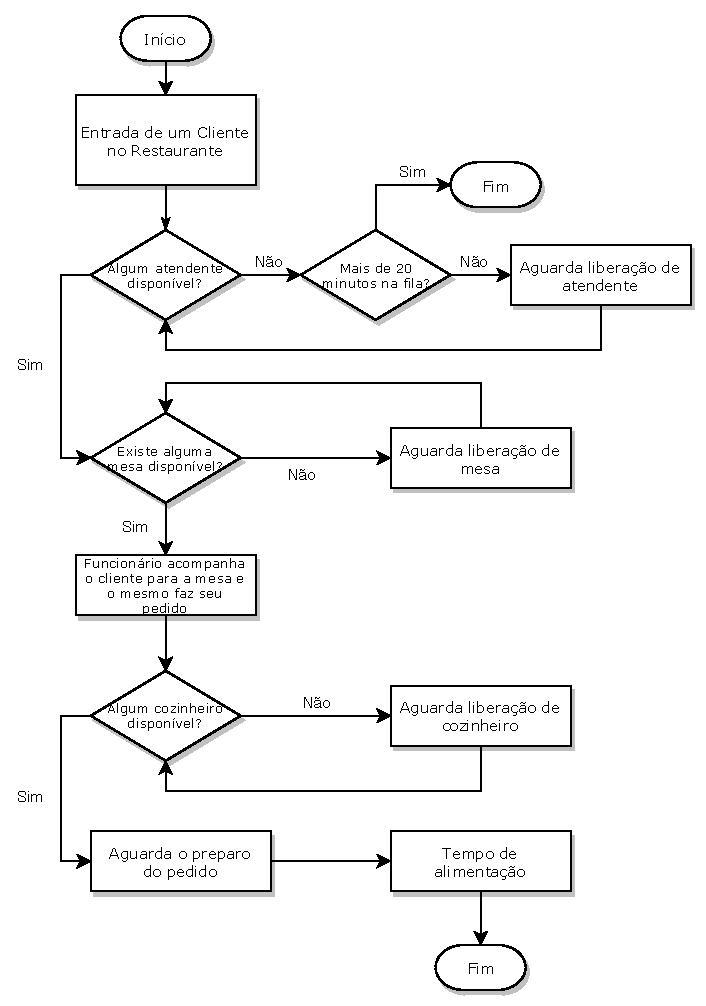
\includegraphics[width=.75\textwidth]{images/Fluxograma/Fluxograma.pdf}
					\caption{Blocos que compõem o modelo do sistema ao qual este trabalho pretende utilizar de base para análises futuras.}
					\label{fig.fluxograma}
				\end{center}
			\end{figure}

			Os principais componentes do sistema são:

			\begin{itemize}
					\item[\textbf{Cliente (Entidade):}] Representa uma pessoa que deseja se alimentar no restaurante. Ela é atendida por apenas um atendente, um cozinheiro e senta-se em apenas uma mesa.
					\item[\textbf{Atendente (Recurso):}] Representa uma pessoa que recebe os clientes na porta do restaurante, encaminhando-as a uma mesa. Ela também é responsável por anotar o pedido do cliente e repassar para os cozinheiros.
					\item[\textbf{Cozinheiro (Recurso):}] Representa uma pessoa que cozinha o prato que um cliente pediu.
					\item[\textbf{Mesa (Recurso):}] Representa uma mesa que é utilizada por um cliente durante o período de realização do pedido pelo cliente até o fim da alimentação do mesmo.
			\end{itemize}

			As variáveis do sistema são:

			\begin{itemize}
				\item[\textbf{Tempo de chegada de clientes:}] determina o intervalo de chegada de clientes no sistema. Incorporado ao modelo através da configuração de um componente de criação de entidades com a distribuição teórica correspondente.
				\item[\textbf{Tempo de preparo das refeições:}] determina o tempo que um cliente aloca um recurso cozinheiro. Incorporado ao modelo através da configuração de um atraso com a distribuição teórica correspondente.
				\item[\textbf{Tempo de alimentação dos clientes:}] determina o tempo, somado ao tempo de preparo da refeição, que um cliente aloca um recurso mesa. Incorporado ao modelo através da configuração de um atraso com a distribuição teórica correspondente.
			\end{itemize}
			
			Os cenários serão representados por meio da permutação dos níveis dos três fatores do modelo, entre eles, a quantidade de atendentes, a quantidade de cozinheiros e a quantidade de mesas.
			A aquisição dos resultados para analise serão extraídos das informações das entidades e dos recursos armazenadas durante o tempo de simulação do modelo.
			Alguns exemplos gerais de informações relevantes são quantidade de entidades criadas, tempo de espera de uma entidade em uma determinada fila, tempo médio que um recurso permanece alocado etc.

		\section{Coleta de Dados}
		\label{sec:coleta}

            Para o processo de simulação, em geral, é necessária a realização de coletas dados de algumas variáveis pertencentes ao domínio do problema.
            Esta é uma etapa de muita importância, uma vez que esses dados serão utilizados na modelagem do comportamento do modelo de simulação.
            Logo, os dados coletados precisam refletir as características do mundo real para que o modelo possa refleti-lo corretamente. 
            
            Incluem-se nesta etapa a síntese estatística dos dados, a identificação e caracterização da melhor distribuição de probabilidade teórica que representa o conjunto de dados coletados e o teste de aderência que confirma se a distribuição teórica representa os dados.
            Para efeitos didáticos, as variáveis tempo de chegada e alimentação dos clientes foram disponibilizadas pelo orientador deste trabalho, sendo dispensável a realização do processo de amostragem de tais variáveis.
            A terceira variável aleatória que influencia o modelo (tempo de preparo dos alimentos) será gerada a partir de uma distribuição uniforme entre 3 e 8 minutos.
            Essa distribuição foi selecionada partindo do princípio de que os pratos servidos no restaurante desse modelo são genéricos e portanto possuem o mesmo tempo de preparo, salvo pequenas variações aleatórias.

            \subsection{Tratamento de Dados e Seleção das Distribuições de Probabilidades}
			\label{subsec:tratamento}
			
				Após recebimento dos dados, os mesmos foram submetidos as análises mencionadas em \ref{sec:sintese} através da ferramenta \textit{Input Analyzer}.
				Houve necessidade de solicitar uma nova amostra para a variável tempo de chegada, uma vez que a primeira fornecida era insuficiente.
				Os resultados das análises após o recebimento de amostras suficientes para ambas as variáveis são apresentadas abaixo.
				
				\begin{itemize}

					\item{\textbf{Tempo de chegada em segundos:}}
					\begin{itemize}
						\item{\textbf{Tamanho da amostra:}} $225$
						\item{\textbf{Número de classes:}} $15$
						\item{\textbf{Média:}} $84.1$
						\item{\textbf{Desvio padrão:}} $8.05$
						\item{\textbf{Distribuição de Probabilidade:}} $64 + 41 \times BETA(2.7, 2.79)$
					\end{itemize}

					\item{\textbf{Tempo de alimentação em minutos:}}
					\begin{itemize}
						\item{\textbf{Tamanho da amostra:}} $50$
						\item{\textbf{Número de classes:}} $7$
						\item{\textbf{Média:}} $34.9$
						\item{\textbf{Desvio padrão:}} $9.75$
						\item{\textbf{Distribuição de Probabilidade:}} $23 + GAMMA(7.95, 1.49)$
					\end{itemize}

				\end{itemize}

            \subsection{Testes de Aderência}
			\label{subsec:testes}
			
			De forma semelhante a \ref{subsec:tratamento} foi utilizada a ferramenta \textit{Input Analyzer} para a realização dos cálculos mencionados em \ref{sec:inferencia}.
			Para as distribuições teóricas com o menor erro quadrático, foi realizado o teste de hipótese não paramétrico descrito em \ref{sec:inferencia}.
			Através dos graus de liberdade para as amostras, desconsiderando as classes com frequência insuficiente para o teste de aderência, foram obtidos os valores de $\chi$-Quadrado crítico para 95\% de confiança.
			Dessa maneira, como ambos erros quadráticos são menores que o erro crítico é possível aceitar a hipótese nula, ou seja, as distribuições teóricas representam os dados de forma significante.
			
			\begin{itemize}

				\item{\textbf{Tempo de chegada:}}
				\begin{itemize}
					\item{\textbf{Graus de liberdade:}} $10$
					\item{\textbf{Tabela $\chi$-Quadrado crítico:}} $3.94$
					\item{\textbf{Erro quadrático:}} $0.003321$
				\end{itemize}

				\item{\textbf{Tempo de alimentação:}}
				\begin{itemize}
					\item{\textbf{Graus de liberdade:}} $3$
					\item{\textbf{Tabela $\chi$-Quadrado crítico:}} $0.35$
					\item{\textbf{Erro quadrático:}} $0.019768$
				\end{itemize}

			\end{itemize}

		\section{Tradução do Modelo}
		\label{sec:traducao}

			O Código \ref{cod.codigo} foi gerado automaticamente pelo Arena a partir do modelo, que por sua vez é exibido na Figura \ref{fig.modelo} e contêm a definição formal de cada um dos componentes do sistema.

			\vspace{.5 cm}			

			\lstinputlisting[label = cod.codigo, title = \textbf{Código 3.5:} código em SIMAN gerador do modelo no Arena., captionpos = b]{./images/Codigo/codigo.cpp}
			\lstset{
				tabsize=1,
				language=verilog,
				basicstyle=\scriptsize\ttfamily,
				breaklines=true,
				showstringspaces=false,
				frame=single,
				numbers=left
			}

			\begin{figure}[]
				\begin{center}
					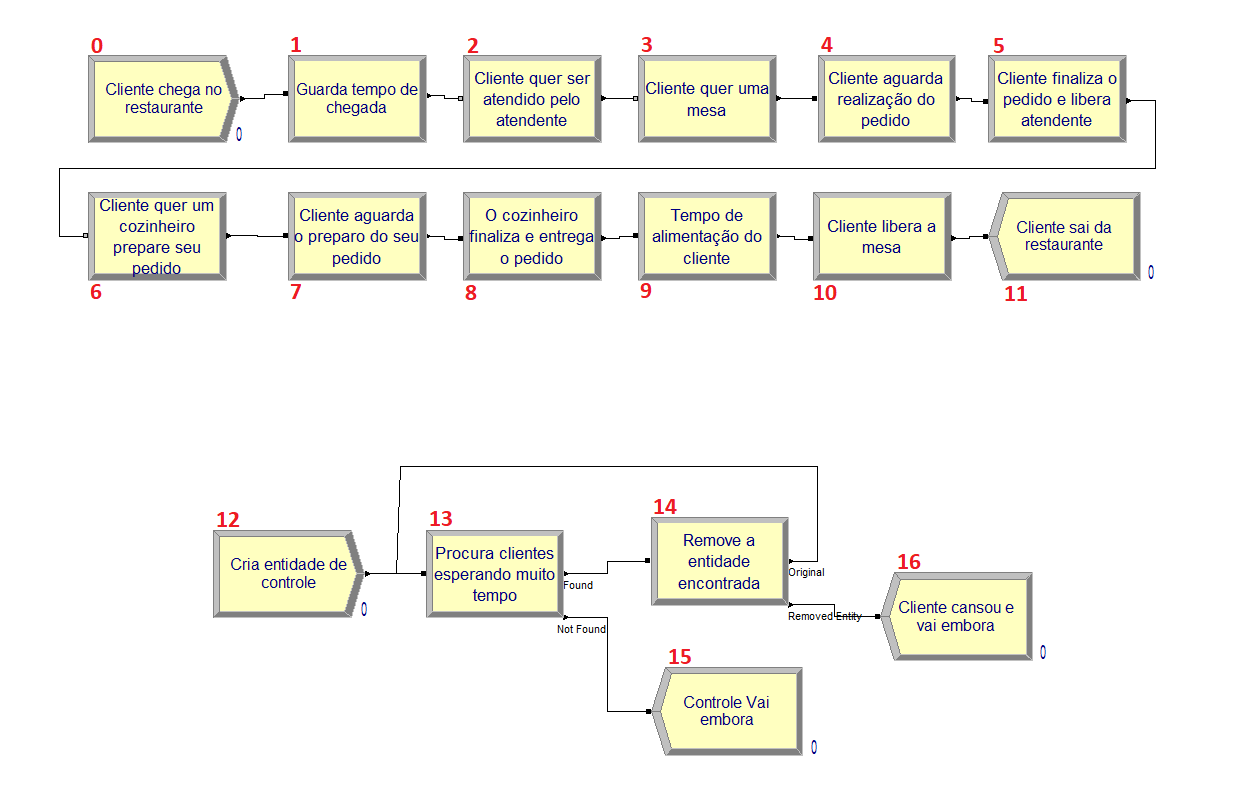
\includegraphics[width=\textwidth]{./images/Figures/model_v.png}
					\caption{Modelo do sistema (ARENA).}
					\label{fig.modelo}
				\end{center}
			\end{figure}

			A incorporação da variável ``tempo de chegada de clientes`` é realizada no componente \textit{CREATE} (linha 5 - componente 0) através da função de distribuição identificada na Subseção \ref{subsec:tratamento}.
			A variável ``tempo de preparo das refeições`` é representada pelo \textit{DELAY} (linha 79 - componente 7).
			De forma similar, a variável ``tempo de alimentação dos clientes`` também é definida através de um \textit{DELAY} (linha 91 - componente 9), seguindo a distribuição correspondente.

			Cada fator do sistema é representado por um único recurso, dentre eles, Atendentes, Cozinheiros e Mesas.
			Desta forma, é possível que o \textit{Process Analyser} (programa auxiliar utilizado para a realização do projeto experimental) alterne a capacidade dos recursos entre o nível mínimo e máximo, de modo que seja possível a criação dos $2^3$ cenários.
			A alocação e desalocação do recurso Atendentes são realizadas nos componente 2 e 5 (linhas 25 e 58), respectivamente.
			Para o recursos Cozinheiros, a alocação é realizada no componente 6 (linha 67) e a desalocação no componente 8 (linha 85).
			Finalmente, o recurso Mesas é alocado após da obtenção do recurso Atendente, no componente 3 (linha 39) e desalocado após a liberação do recurso Cozinheiro, componente 10 (linha 97).

			Durante a simulação do modelo foram armazenados dados sobre as entidades do tipo Cliente e Atendentes para que seja possível a obtenção de informações relevantes a análise.
			Assim posto, a quantidade de clientes que entraram no restaurante pode ser obtida a partir da variável \textit{Cliente chega no restaurante.NumberIn} do \textit{CREATE}, incrementada toda vez que um cliente é criado.
			A quantidade de clientes que foram atendidos pode ser obtida a partir da variável \textit{Atendentes.TotalNumberSeized}, incrementada toda vez que o recurso Atendentes é alocado.
			Por fim, a quantidade de clientes que saíram do restaurante deve ser adquirida a partir da soma das variáveis \textit{NumberOut} dos dois componentes \textit{DISPOSE} de clientes do modelo (\textit{Cliente sai da restaurante} (linha 104 - componente 11) e \textit{Cliente cansou e vai embora} (linha 145 - componente 16)) que representam os clientes satisfeitos e os que desistiram de esperar.

		\section{Verificação}
		\label{sec:verificacao}

			A elaboração do modelo de simulação foi separado em dois fluxos distintos: fluxo de clientes[0..11] e fluxo de controle[12..16], mostrados na Figura \ref{fig.modelo}.
			Os clientes são representados por entidades do modelo que alocam, desalocam e esperam pelos recursos definidos a seguir.
			Os atendentes, por sua vez, são representados por um único recurso, denominado Atendentes, onde a quantidade de atendentes é definida através da capacidade que esse recurso possui.
			Os cozinheiros e mesas, denominados Cozinheiros e Mesas respectivamente, seguem a mesma definição do recurso Atendentes.

			O fluxo de clientes exerce o comportamento de um cliente que consegue ser atendido e saí do estabelecimento satisfeito.
			Inicialmente, a chegada de um cliente é definida pelo componente 0 (\textit{CREATE}) que insere entidades cliente no modelo.
			Em seguida, a espera de um cliente para ser atendido é representado pelo componente 2 (\textit{SEIZE}) que tentará alocar um \textit{slot} do recurso Atendentes.
			Caso não existam atendentes disponíveis, o cliente será inserido em uma fila ordenada pelo tempo de chegada.
			Após a alocação de um \textit{slot} do Atendentes, a entidade tentará alocar um \textit{slot} do recurso Mesas, componente 3 (\textit{SEIZE}), representando o comportamento de encaminhar o cliente a uma mesa disponível.
			Com uma mesa alocada, o componente 4 (\textit{DELAY}) concretiza o comportamento de escolha de refeição do cliente.
			Não precisando mais de um atendente, a entidade cliente libera o recurso no componente 5 (\textit{RELEASE}).
			Posteriormente, a entidade tenta alocar um \textit{slot} do recurso Cozinheiros, efetuado pelo componente 6 (\textit{SEIZE}), esperando numa fila caso não exista nenhum disponível.
			De forma similar a realização do pedido, a entidade cliente permanece por um período de tempo no componente 7 (\textit{DELAY}) aguardando o preparo de sua refeição.
			Ao término do preparo, o cozinheiro é liberado pelo componente 8 (\textit{RELEASE}).
			Com a refeição pronta, a entidade cliente demora-se no componente 9 (\textit{DELAY}) enquanto alimenta-se.
			Ao final da refeição, a entidade cliente libera o recurso mesa no componente 10 (\textit{RELEASE}) e saí satisfeito do restaurante através do componente 11 (\textit{DISPOSE}).

			Em paralelo, o fluxo de controle executa o critério de desistência de clientes que esperam muito tempo para serem atendidos.
			A execução é realizada por entidades de controle criadas de tempos em tempos (componente 12) que realizam uma busca (componente 13) na fila \textit{Cliente quer ser atendido pelo atendente.Queue}.
			Toda entidade que esteja a mais de 20 minutos possui 20\% de chance de desistir e ir embora.
			Caso a entidade de controle encontre um cliente que deseja ir embora, então este cliente será removido da fila (através do componente 14) e, portanto, sairá do sistema (componente 16).
			Após finalizar as verificações, a entidade de controle é removida do sistema (componente 15).

		\section{Validação}
		\label{sec:validacao}

			De acordo com o que foi dito na Subseção \ref{subsec:testeStudent}, foi utilizado o teste t-Student para comparar as médias do modelo simulado com as médias do sistema real.
			Para isso, neste trabalho $H_0$ consiste na inexistência de diferença entre as médias, ou seja, as médias das variáveis observadas condizem com o comportamento do sistema real e, de forma contrária, assume-se em $H_1$ que as médias sejam diferentes.
			Os testes referentes a cada variável observada, descritos a seguir, utilizam um nível de confiança de 95\% e critério bi-caudal.

			Os dados do modelo, mostrados nas Tabelas \ref{table:modeloErrado} e \ref{table:modeloCorreto}, foram gerados através da simulação do modelo em 30 replicações de 8 horas cada.
			De forma semelhante, os dados do sistema real, mostrados na Tabela \ref{table:modeloReal}, foram entregues pelo professor responsável supondo os mesmos parâmetros.
			Assim, foi possível a realização de uma análise do modelo em relação ao sistema real.

			\begin{table}[!ht]
				\centering
				\begin{tabular}{l|c|c}
					\rowcolor{gray!70} Variável 						   & Média   & Desvio Padrão \\
					\rowcolor{gray!20} Quantidade de clientes que chegaram & 343.1   & 0.84 		 \\
					\rowcolor{gray!40} Quantidade de clientes que saíram   & 268.83  & 2.35 		 \\
					\rowcolor{gray!20} Quantidade de clientes atendidos    & 97.3667 & 1.01
				\end{tabular}
				\caption{primeiros resultados do modelo de simulação.}
				\label{table:modeloErrado}
			\end{table}

			\begin{table}[!ht]
				\centering
				\begin{tabular}{l|c|c}
					\rowcolor{gray!70} Variável 						   & Média   & Desvio Padrão \\
					\rowcolor{gray!20} Quantidade de clientes que chegaram & 309.73  & 0.44 		 \\
					\rowcolor{gray!40} Quantidade de clientes que saíram   & 280.17  & 1.27 		 \\
					\rowcolor{gray!20} Quantidade de clientes atendidos    & 93.83   & 0.85
				\end{tabular}
				\caption{resultados finais do modelo de simulação.}
				\label{table:modeloCorreto}
			\end{table}

			\begin{table}[!ht]
				\centering
				\begin{tabular}{l|c|c}
					\rowcolor{gray!70} Variável 						   & Média   & Desvio Padrão \\
					\rowcolor{gray!20} Quantidade de clientes que chegaram & 310  	 & 1.2 			 \\
					\rowcolor{gray!40} Quantidade de clientes que saíram   & 280  	 & 2.1 			 \\
					\rowcolor{gray!20} Quantidade de clientes atendidos    & 94.1 	 & 1.9
				\end{tabular}
				\caption{resultados do modelo real fornecidos pelo professor responsável.}
				\label{table:modeloReal}
			\end{table}

			Os primeiros testes utilizando os dados da Tabela \ref{table:modeloErrado} em relação aos dados reais permitiram rejeitar $H_0$ em todas as variáveis, demonstrando que o modelo não correspondia ao sistema real.
			Desta forma, algumas alterações no modelo tiveram de ser realizadas, tais como o aumento no valor do parâmetro correspondente ao deslocamento da função de distribuição da variável ``tempo de chegada de clientes`` ($73 + 41 \times BETA(2.7, 2.79)$), aumento no valor da variável ``tempo de realização do pedido`` ($UNIF(3, 8)$) e, por fim, aumento da probabilidade de um cliente ir embora do restaurante (de 1\% para 20\%).

			Após a realização de novas execuções do modelo, sob as mesmas condições descritas anteriormente, os dados da Tabela \ref{table:modeloCorreto} foram obtidos.
			Por fim, todas as variáveis do modelo alterado passaram no teste de validação, onde os resultados obtidos podem ser vistos abaixo:

			\begin{itemize}
				\item{\textbf{Quantidade de clientes que chegaram:}}
				\begin{itemize}
					\item{Variância ponderada:} $0.233352$
					\item{Graus de liberdade:} $37$
					\item{\textit{t} observado:} $-1.15705$
					\item{\textit{t} crítico:} $+/- 2.02619246$
					\item{Resultado:} Aceita $H_0$
				\end{itemize}

				\item{\textbf{Quantidade de clientes que saíram:}}
				\begin{itemize}
					\item{Variância ponderada:} $0.448066$
					\item{Graus de liberdade:} $48$
					\item{\textit{t} observado:} $0.379408$
					\item{\textit{t} crítico:} $+/- 2.01063476$
					\item{Resultado:} Aceita $H_0$
				\end{itemize}

				\item{\textbf{Quantidade de clientes que atendidos:}}
				\begin{itemize}
					\item{Variância ponderada:} $0.380022$
					\item{Graus de liberdade:} $41$
					\item{\textit{t} observado:} $-0.710485$
					\item{\textit{t} crítico:} $+/- 2.01954097$
					\item{Resultado:} Aceita $H_0$
				\end{itemize}
			\end{itemize}

		\section{Projeto Experimental e Experimentação}
		\label{sec:experimentos}

			A realização dos diversos experimentos necessários para a análise posterior dos dados é feita através da ferramenta \textit{Process Analyzer}, pertencente ao conjunto do \textit{Arena}.
			Para isso, foi utilizado o modelo, descrito nas seções anteriores, criando cenários específicos com valores mínimos e máximos dos fatores que interferem nas variáveis de interesse do projeto.
			Com a finalidade de obter amostras com erro experimental, empregou-se o projeto experimental $2^k$ com replicações.
			
			Inicialmente, os recursos do sistema foram representados por conjuntos, mas ao definir os experimentos no \textit{Process Analyzer}, foi observado que a ferramenta aceita apenas modificações na capacidade de recursos únicos, não permitindo a alteração da quantidade de recursos de um conjunto.
			Caso utilizássemos conjuntos como especificado originalmente, a adição manual de 50 mesas dificultaria a realização dos experimentos e na sua corretude, implicando na realização manual de todos os cenários.
			Como solução, os conjuntos de recursos foram simplificados para um único recurso com capacidade variável, possibilitando a criação e execução dos cenários através do \textit{Process Analyzer}.
			Assim, serão utilizados três fatores de entrada para cada cenário, o recurso que representa a quantidade de mesas no restaurante (Mesas), outro representando a quantidade de atendentes (Atendentes) e, por fim, um representando a quantidade de cozinheiros (Cozinheiros).

			O nível mínimo do fator Mesas é 30, representando a retirada de 40\% das mesas do estabelecimento, enquanto o nível máximo é 50 (quantidade atual de mesas).
			Nos fatores Atendentes e Cozinheiros, o nível mínimo é 1, representando a quantidade atual de funcionários de cada setor e o nível máximo é 5, ou seja, a necessidade de contratar mais atendentes ou cozinheiros.
			Por fim,as combinações desses fatores apresentados acima resulta em oito cenários (três fatores $\,\to\,$ $2^3$ = 8), como mostrado na Figura \ref{fig.experimentos}.
			Cada cenário será replicado 30 vezes, resultando em um total de duzentos e quarenta (240) experimentos.

			\begin{figure}[H]
				\begin{center}
					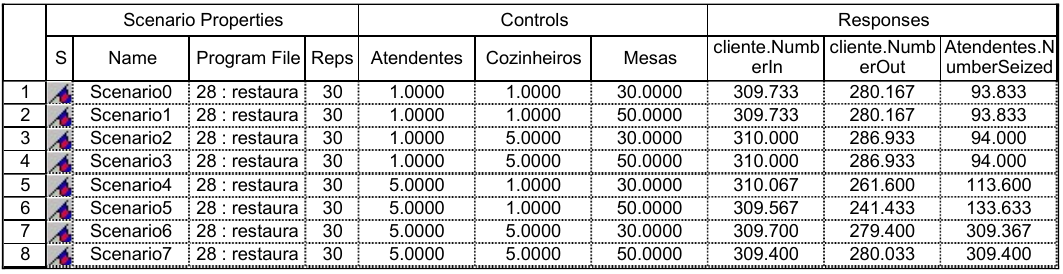
\includegraphics[width=.75\textwidth]{images/ProcessAnalyzer/grade.png}
					\caption{conjunto de $2^3$ experimentos realizados na ferramenta \textit{Process Analyzer}.}
					\label{fig.experimentos}
				\end{center}
			\end{figure}

		\section{Apresentação e Análise Estatísticas dos Resultados}
		\label{sec:apresentacao_analise}

			Após a realização dos $2^k$ experimentos através do \textit{Process Analyzer}, foi realizado um estudo para obter os dados de contribuição dos fatores que influenciam o modelo.
			Para isso, foi utilizado o método visto em aula, onde são obtidos os coeficientes de influência de cada fator e estes, por sua vez, são utilizados para a construção de uma função que permite estimar valores que variam entre o mínimo e máximo desse fator.
			As Tabelas \ref{table:results1}, \ref{table:results2} e \ref{table:results3} mostram os resultados obtidos após os experimentos realizados:

			\begin{table}[!ht]
				\centering
				\begin{tabular}{c|c|c}
					\rowcolor{gray!70} Fator 	& Coeficiente 	& Contribuição 	\\
					\rowcolor{gray!20} A 		& 0.13			& 0.84\%		\\
					\rowcolor{gray!40} B 		& 0.25			& 3.36\%		\\
					\rowcolor{gray!20} C 		& -0.38			& 7.56\%		\\
					\rowcolor{gray!40} AB 		& -0.25			& 3.36\%		\\
					\rowcolor{gray!20} AC 		& -0.38			& 7.56\%		\\
					\rowcolor{gray!40} BC 		& -0.25			& 3.36\%		\\
					\rowcolor{gray!20} ABC 		& -0.25			& 3.36\%		\\
				\end{tabular}
				\caption{coeficientes obtidos após a realização de 2 replicações para cada um dos cenários de estudo para o número de clientes que chegaram. Onde A é o número de atendentes, B é o número de cozinheiros e C é o número de mesas.}
				\label{table:results1}
			\end{table}

			A função de combinação de fatores para a quantidade de clientes que chegaram é:

			\begin{center}
				\large{$FClienteChegaram = 0.13 \times A + 0.25 \times B - 0.38 \times C - 0.25 \times AB - 0.38 \times AC - 0.25 \times BC - 0.25 \times ABC + 310.13$}
			\end{center}

			\begin{table}[!ht]
				\centering
				\begin{tabular}{c|c|c}
					\rowcolor{gray!70} Fator 	& Coeficiente 	& Contribuição 	\\
					\rowcolor{gray!20} A 		& -8.25			& 33.74\%		\\
					\rowcolor{gray!40} B 		& 9.25			& 42.41\%		\\
					\rowcolor{gray!20} C 		& -2.5			& 3.1\%			\\
					\rowcolor{gray!40} AB 		& 4.5			& 10.04\%		\\
					\rowcolor{gray!20} AC 		& -2.5 			& 3.1\%			\\
					\rowcolor{gray!40} BC 		& 2.5			& 3.1\%			\\
					\rowcolor{gray!20} ABC 		& 2.5			& 3.1\%			\\
				\end{tabular}
				\caption{coeficientes obtidos após a realização de 2 replicações para cada um dos cenários de estudo para o número de clientes que saíram. Onde A é o número de atendentes, B é o número de cozinheiros e C é o número de mesas.}
				\label{table:results2}
			\end{table}

			A função de combinação de fatores para a quantidade de clientes que saíram é:

			\begin{center}
				\large{$FClienteSairam = -8.25 \times A + 9.25 \times B - 2.5 \times C + 4.5 \times AB - 2.5 \times AC + 2.5 \times BC + 2.5 \times ABC + 273.5$}
			\end{center}

			\begin{table}[!ht]
				\centering
				\begin{tabular}{c|c|c}
					\rowcolor{gray!70} Fator 	& Coeficiente 	& Contribuição 	\\
					\rowcolor{gray!20} A 		& 60.31			& 45.48\%		\\
					\rowcolor{gray!40} B 		& 45.81			& 26.24\%		\\
					\rowcolor{gray!20} C 		& 2.06			& 0.05\%		\\
					\rowcolor{gray!40} AB 		& 47.31			& 27.99\%		\\
					\rowcolor{gray!20} AC 		& 2.06			& 0.05\%		\\
					\rowcolor{gray!40} BC 		& -2.44			& 0.07\%		\\
					\rowcolor{gray!20} ABC 		& -2.44			& 0.07\%		\\
				\end{tabular}
				\caption{coeficientes obtidos após a realização de 2 replicações para cada um dos cenários de estudo para o número de clientes atendidos. Onde A é o número de atendentes, B é o número de cozinheiros e C é o número de mesas.}
				\label{table:results3}
			\end{table}

			A função de combinação de fatores para a quantidade de clientes atendidos é:

			\begin{center}
				\large{$FClienteChegaram = 60.31 \times A + 45.81 \times B + 2.06 \times C + 47.31 \times AB + 2.06 \times AC - 2.44 \times BC - 2.44 \times ABC + 156.31$}
			\end{center}

			A Tabela \ref{table:resultsValues} mostra os valores de contribuição total dos fatores para cada uma das respostas obtidas a partir do projeto de experimentos.
			Como é possível observar, os fatores avaliados, basicamente, não influenciam o número de clientes que chegaram.
			Isso ocorre devido ao fato de que todos os fatores avaliados influenciam a entidade cliente apenas depois de sua criação, ou seja, quando ela já está no fluxo interno do modelo.
			Diferentemente do caso anterior, os fatores tem grande influência no número de cliente atendidos e que saíram do modelo.
			Isso ocorre pelo fato de que o gargalo do modelo consiste, essencialmente, no número máximo de atendentes e cozinheiros que podem ser alocados simultaneamente, já que estes são os recursos mais disputados dentre o conjunto necessário para que o cliente passe do início ao fim do fluxo estabelecido no modelo.


			\begin{table}[!ht]
				\centering
				\begin{tabular}{c|c|c|c}
					\rowcolor{gray!70} Variável 					& $SS_{modelo}$	& $SS_{erro}$	& $SS_{total}$	\\
					\rowcolor{gray!20} Nº de clientes que chegaram 	& 29.41\%		& 70.56\%	& 29.75			\\
					\rowcolor{gray!40} Nº de clientes que saíram	& 98.57\%		& 1.43\%	& 3,228.00		\\
					\rowcolor{gray!20} Nº de clientes atendidos		& 99.96\%		& 0.04\%	& 127,975.44	\\
				\end{tabular}
				\caption{porcentagem de contribuição do modelo em relação ao modelo real.}
				\label{table:resultsValues}
			\end{table}

		\section{Identificação das Melhores Soluções}
		\label{sec:identificacao}

			Assim como pode ser observado na Figura \ref{fig.experimentos}, olhando os cenários onde houve apenas alterações no número de mesas, é possível notar que a remoção de 40\% delas tem uma influência insignificante no número de clientes atendidos.
			Isso acontece pois os demais recursos são em quantidade bem menores e necessário para que o cliente possa chegar a alocar uma mesa.
			Essa característica do modelo fica mais clara quando analisados os resultados obtidos nas Tabelas \ref{table:results1}, \ref{table:results2} e \ref{table:results3}.
			Como pode-se notar, em todos os casos onde aparece o fator C (número de mesas) a influência no modelo é relativamente pequena se comparada com os demais.
			Portanto, é possível concluir que a Hipótese 2, formulada em \ref{sec:hipoteses}, pode ser aceita como verdadeira.

			Ao contrário do fator avaliado anteriormente, o número de atendentes e cozinheiros influenciaram consideravelmente os resultados obtidos nas análises.
			Comparando-se os resultados obtidos nos cenários 1 e 3 e nos cenários 1 e 5, percebe-se que a alteração apenas no número de atendentes ou só o número de cozinheiros o impacto não é tão significativo.
			Isso ocorre pois ambos os recursos são essenciais para o cliente e o fato de aumentar a disponibilidade de apenas um recurso faz com que o gargalo do modelo mude de lugar, ou seja, quando aumentado apenas o número de atendentes, o recurso Cozinheiros passa a ser mais disputado, ocorrendo o inverso quando aumentado apenas o número de cozinheiros.
			Assim, quando a quantidade de ambos os recursos são aumentados simultaneamente (cenários 6 e 7), nota-se que o número de cliente atendidos aumenta quase 200\% em relação ao valor obtido nos demais cenários.
			Devido a isso, a Hipótese 1, também formulada em \ref{sec:hipoteses}, pode ser rejeitada, uma vez que a contratação apenas de cozinheiros não implica no aumento em dobro do número de clientes atendidos.

			Logo, a melhor solução encontrada para o problema proposto neste documento é a contratação simultânea de 4 novos atendentes e cozinheiros, pois como é possível verificar nos resultados dos cenários 6 e 7, foram os que mais aumentaram o número de clientes atendidos.
			Além disso, a remoção de 40\% das mesas, por não impactar nos resultados, podem ser removidas em vista da instalação de palco para eventos no restaurante.

	\chapter{Conclusões}
	\label{cap:conclusoes}

		Em diversas situações do cotidiano de um cientista da computação surgem problemas que o faz por em prova seus conhecimentos e habilidades.
		Diversas abordagens podem ser utilizadas para que se possa encontrar uma solução para tais problemas.
		No entanto, é de extrema importância ter ferramentas (e o conhecimento necessário para utilizá-las) que permitam obter a solução de acordo com as restrições tecnológicas, temporais, de eficiência entre outras, as quais são impostas no processo de busca por soluções.
		Dessa maneira, é importante identificar qual o propósito de cada ferramenta e de que maneira pode ser utilizada.
		Nesse sentido, é extremamente válido ter como ferramenta o conhecimento sobre simulação de sistemas, como utilizá-la, suas restrições e os melhores meios para se atingir o objetivo em questão.
		Tal conhecimento permite solucionar problemas que envolvem a construção de modelos que representam situações comuns no dia-a-dia com a finalidade de simulá-los e obter estatística relevantes que possam predizer ou até mesmo estimar determinados comportamentos ou propriedades.

		Para se utilizar os recursos providos por modelos computacionais para simulação de sistemas, é necessário que, primeiramente, tenha-se conhecimentos sobre métodos e modelos estatísticos.
		Por capturar comportamentos observáveis no mundo real, modelos de simulação geralmente não são determinísticos, podendo gerar respostas diferentes a cada vez que são executados.
		Por conta disso, para modelar o mundo real de forma a capturar as características essenciais a serem representadas, é necessário os conhecimentos de distribuições de probabilidades, cálculo de métricas de dispersão e valor central, testes de hipóteses entre outros.
		Com tais conhecimentos estatísticos é possível avaliar e verificar o modelo desenvolvido com a finalidade de confrontá-lo com o modelo real e determinar se o mesmo é representativo e pode ser utilizado para obter as conclusões desenvolvidas.

		Este trabalho, fazendo uso dos conhecimentos adquiridos ao longo da disciplina, buscou modelar um empreendimento do ramo alimentício e solucionar um problema básico mas recorrente.
		Aplicando das técnicas e modelos consolidados nas aulas, foi possível a extração dos principais componentes que influenciam o modelo fictício proposto e, dessa maneira, criar um modelo de simulação que o representasse.
		Além disso, o uso de ferramentas de simulação e estatística, tais como o Arena e \textit{Input Analyser}, possibilitou obter uma visão geral sobre diversas características que podem ser representadas por modelos de simulação.
		Embora certos pontos não tenham sido explorados neste trabalho (características mais complicadas de serem simuladas, tais como nos modelo físicos) os conhecimentos adquiridos são de grande importância para construir uma base que sirva para direcionar a solução de problemas mais complexos.

		Portanto, modelos de simulação podem ser utilizados para solucionar problemas interessantes e de grande relevância, tanto no contexto profissional quanto acadêmico, possibilitando a aplicação e exploração de diversos conceitos abordados ao longo da graduação em ciências da computação.

	\backmatter
	\appendix

	\bibliographystyle{apalike}
	\bibliography{referencias}

\end{document}
